\documentclass[conference]{IEEEtran}
\IEEEoverridecommandlockouts
% The preceding line is only needed to identify funding in the first footnote. If that is unneeded, please comment it out.
\usepackage{cite}
\usepackage{amsmath,amssymb,amsfonts}
\usepackage{algorithmic}
\usepackage{graphicx}
\graphicspath{ {./images/} }
\usepackage{textcomp}
\usepackage{xcolor}
\def\BibTeX{{\rm B\kern-.05em{\sc i\kern-.025em b}\kern-.08em
    T\kern-.1667em\lower.7ex\hbox{E}\kern-.125emX}}
\begin{document}

\title{Acoustic Crack Detection in Material Coupons Using a Deep Convolutional Neural Network
}

\author{\IEEEauthorblockN{Sarah Malik}
\IEEEauthorblockA{\textit{Mechanical \& Computational Engr.} \\
\textit{Drexel University}\\
Philadelphia, PA, USA \\
sm3658@drexel.edu}
\and
\IEEEauthorblockN{Michael Shenoda}
\IEEEauthorblockA{\textit{AI and Machine Learning} \\
\textit{Drexel University}\\
Nashville, TN, USA \\
michael.shenoda@drexel.edu}
\and
\IEEEauthorblockN{Jeremy Fernsler}
\IEEEauthorblockA{\textit{Computer Science} \\
\textit{Drexel University}\\
Glendale, CA, USA \\
jfernsler@drexel.edu}
\and
}

\maketitle

\begin{abstract}
We present a method for detecting structural cracks in a material using acoustic data analyzed by a convolutional neural network (CNN). Material fatigue leading to cracks and faults is a serious problem in vehicles, infrastructure, and many other structures. Work has already been done to analyze the passive signals from MEMs piezo sensors fixed to a surface \cite{b1}. Our method takes the captured waveform from a material sample under load, converts the waveform into frequency space, and passes it through a classifying CNN to detect whether or not the sample contains a crack. We demonstrate the accuracy of such a system and assess the viability of a CNN for acoustic crack detection.
\end{abstract}

\section{Introduction}

As a material undergoes external load, an understanding of fatigue is critical before catastrophic damage. Acoustic Emission provides a sensing methodology to detect the micro structure changes as external load is applied. As the material is loaded in tension, the vibrations can be detected using an acoustic sensor and converted into a voltage waveform. Once a metal or any material begins to fail these vibrations will change because the structure of the material has been compromised. There has been quite a bit of research on music classification \cite{b2} and event detection \cite{b3} in acoustic signals using deep CNNs, and we are going to apply some of these techniques to determine if a trained model can distinguish between a non-cracked or cracked material sample placed under load in laboratory conditions.

\section{Data}
\subsection{Data Acquisition}
Compact Tension (CT) specimens were manufactured form a 4mm thick Aluminum 2024 Alloy plate in accordance with ASTM E1820 and ASTM E647\cite{b5,b6}. In 2024 aluminum alloy, the elemental percentages are 4.4\% Cu, 1.5\% Mg, and 0.6\% Mn, nominally \cite{b7}. The specimen was loaded under quasi-static conditions with a displacement rate of 0.5 mm/min until crack initiation (Figure~\ref{setup}). Acoustic Emission (AE) signals were acquired during the mechanical loading of the specimen in accordance with ASTM E976 \cite{b8}. Hit Definition Time (HDT) is a timing parameter used to trigger the end of waveform capture \cite{b9}. After the hit is complete, the Hit Lockout Time (HLT) value provides a programmable delay before another event can be triggered on the respective channel and Peak Definition Time (PDT) indicates the window of time in which a new peak amplitude can be defined \cite{b9}. For this test, the HDT, HLT, and PDT were 600 µs, 600µs, 200µs, respectively.  

The sensors were bonded to the surface using hot glue and the received signals were amplified using 2/4/6-AST™ pre-amplifiers. A threshold of 45 dB was used that minimized the recording of unwanted noise such as mechanical vibrations introduced by the hydraulic testing machine. The recorded signals were band-pass filtered in the frequency range of 100 kHz–1 MHz and a sampling rate of 5 MHz was utilized. Prior to mechanical loading pencil-lead break tests were carried out to calibrate the response of the AE sensors. 

\begin{figure}[htbp]
\centerline{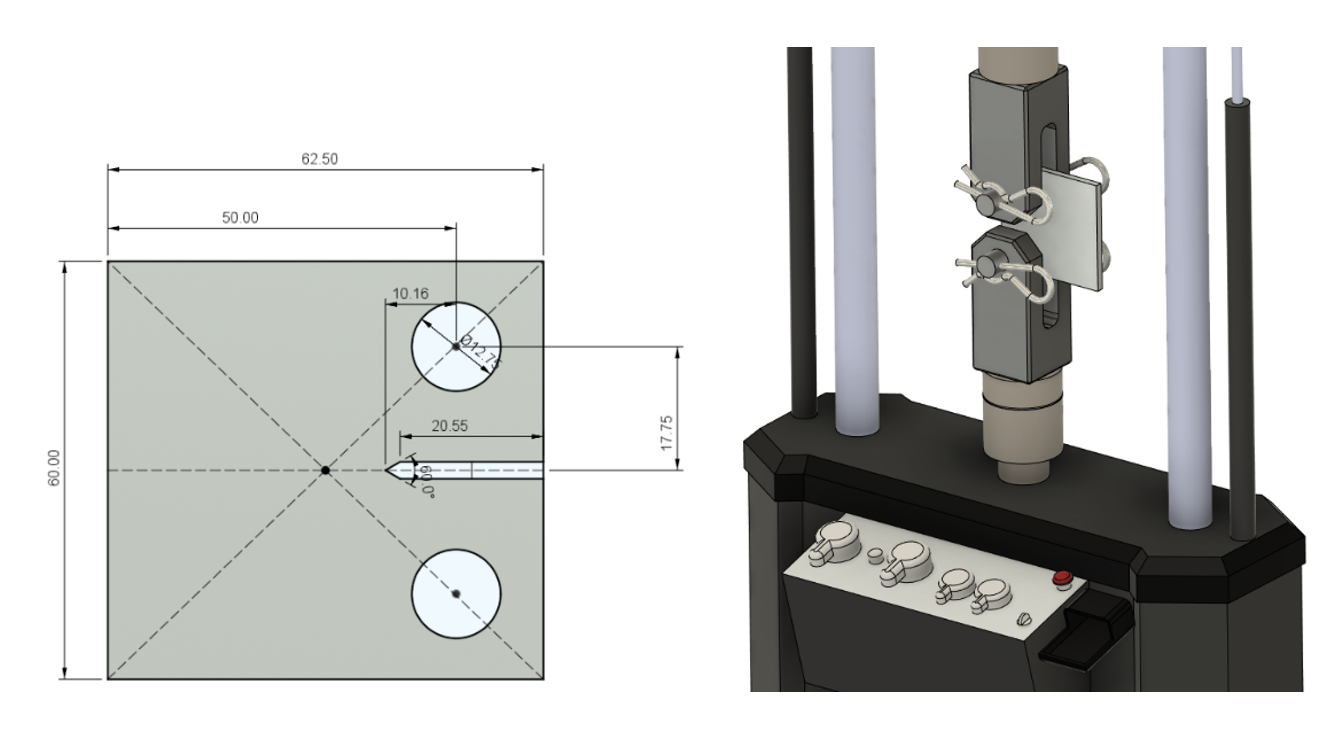
\includegraphics[width=.5\textwidth]{images/setup.png}}
\caption{Test Setup}
\label{setup}
\end{figure}

\subsection{Data Pre-Processing}

The afore mentioned test setup results in individual waveforms saved in plain text files consisting of just over 6000 samples each up to and after the crack as developed. The load value is recorded simultaneously and a severe drop in load value can be marked as a fully developed crack appearing (Figure~\ref{load_chart}). The time at which this drop occurs is recorded and we can use this to label our data as un-cracked (pre-drop) or cracked (post-drop).

For our purposes, we need to collect the data and do a minimal amount of pre-processing. We had access to over 30,000 individual waveform files collected over two tests. The most active channel (of 3 possible) was chosen from each test as the best candidate. Each file is read in, and relevant data is stripped from the headers such as time, which sensor channel is being read, and the sequential number of each waveform as it was collected (Figure~\ref{waveform}). The data was stored in a Pandas dataframe and the crack time (determined by the aforementioned method) was used to label each waveform. \\

\begin{figure}[htbp]
\centerline{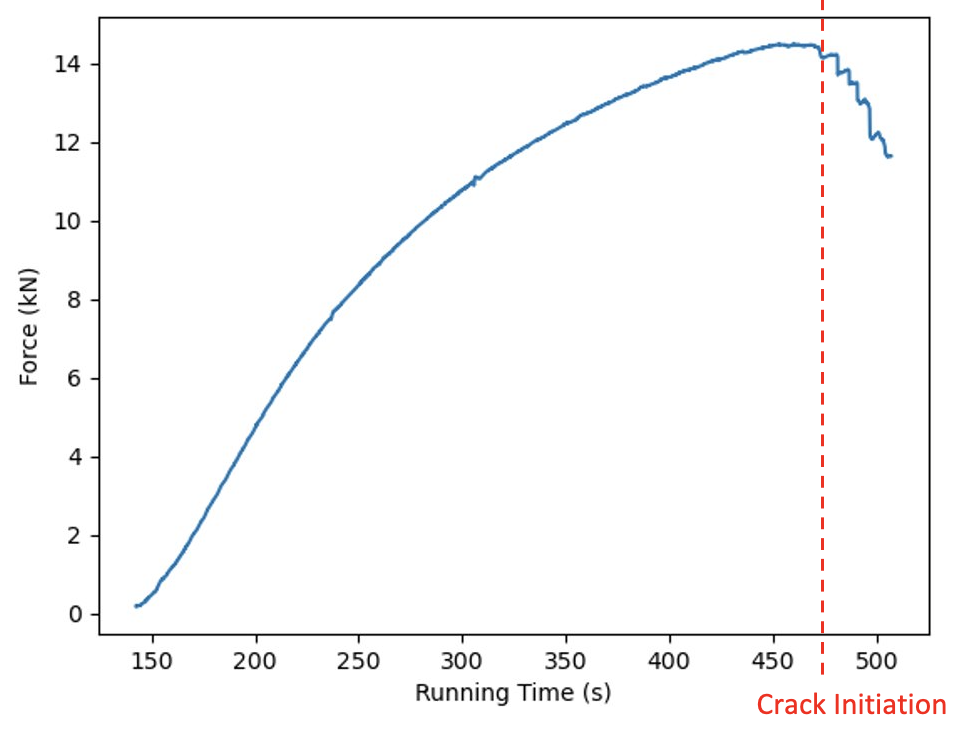
\includegraphics[width=.5\textwidth]{images/force_chart.png}}
\caption{Load vs Time collected during the test. Sudden drop marked with crack initiation. This time was noted for each sample set for the purpose of labeling.}
\label{load_chart}
\end{figure}

A column was created to hold the entropy value for each waveform as this was the measurement used within the lab to attempt to identify when a crack moment happened. Prior work \cite{b1} had previously used the entropy value of the waveform to assess potential damage. While we had some hope to inject this value along side features determined by the CNN \cite{b4}, this did not provide any advantage to the training and was abandoned. A further look at the entropy values between crack and non-crack samples show little to no deviation. While entropy may be useful in determining the \emph{moment} of the crack, using it to differentiate between cracked and non-cracked samples appears far less useful.

The waveforms often contained long stretches of zero values where the tension machine was not applying force and thus creating no new data from the sensor. A new column was created in the dataframe which contained the waveform with stripped zeros - this would become our primary source of data for the project (Figure~\ref{waveform_noz}). This dataframe is pickled for storage and quick reads for training.

After selecting proper samples and labeling it, we had 1665 total crack samples and several thousand non-crack samples. We shuffled all non-crack samples and selected a matching 1665 at random for a total training set of 3330 labeled waveforms, each containing at least 3000 wave samples for each observation. Additionally, we reduced our training set to 500 of each crack and non-crack samples in the interest of the amount of time it takes to train our models. For example, with the full data set, a model setup as seen in Table~\ref{tab1} took approximately 37 minutes per epoch to train. For our allotted window of time we chose to prioritize iteration and evaluation over a larger dataset.

\begin{figure}[htbp]
\centerline{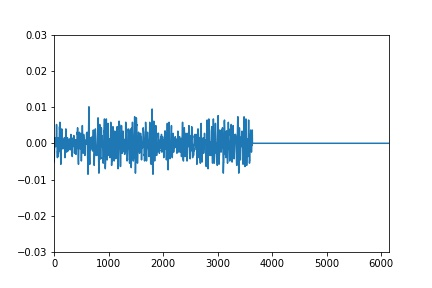
\includegraphics[width=.5\textwidth]{images/data/waveform_153_zeros.jpg}}
\caption{Original waveform (A) sample.}
\label{waveform}
\end{figure}

\begin{figure}[htbp]
\centerline{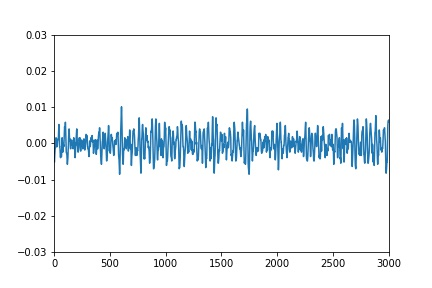
\includegraphics[width=.5\textwidth]{images/data/waveform_153_nozeros.jpg}}
\caption{Waveform (A) with zero data stripped and truncated to 3000 samples.}
\label{waveform_noz}
\end{figure}

\begin{table}[htbp]
\caption{Non-Final CNN layer format 01}
\begin{center}
\begin{tabular}{|c|c|c|}
\hline
\textbf{Layer}&\textbf{Type}&\textbf{Size} \\
\cline{2-3} 
\hline
 0 & InputWaveformLayer & \\
 1 & ConvolutionalLayer & (in:1 out:32 K-5x5) \\
 2 & TanhLayer & \\
 3 & ReLuLayer & \\
 4 & FlattenLayer & \\
 5 & FullyConnected & (492032, 32) \\
 6 & TanhLayer & \\
 7 & FullyConnected & (32, 2) \\
 8 & SigmoidLayer & \\
 9 & SoftmaxLayer & \\
 Objective & CrossEntropy & \\
\hline
\end{tabular}
\label{tab1}
\end{center}
\end{table}

\subsection{Data Within the Model}

The no-zero waveforms are read in and an evenly distributed 80/20 split is generated
for training and validation purposes. We created an WaveformInputLayer which
takes a waveform and casts it to frequency space as a Mel Spectrogram using a
Short Time Fast Fourier Transform (STFFT) (Figure~\ref{melspec}). The window of time used by the STFFT
\begin{figure}[htbp]
\centerline{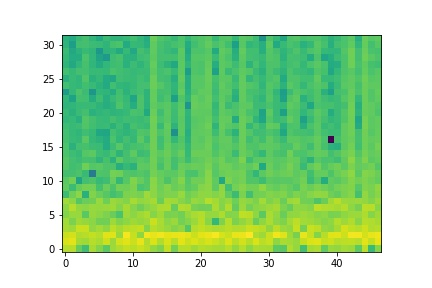
\includegraphics[width=.5\textwidth]{images/data/spectrogram_153.jpg}}
\caption{Mel Spectrogram of waveform (A) Shown here in false color. Actual Spectrogram is a single channel of data in a 2d matrix.}
\label{melspec}
\end{figure}

\begin{figure}[htbp]
\centerline{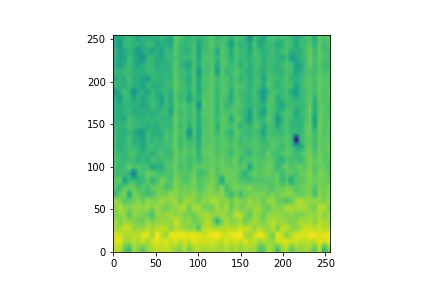
\includegraphics[width=.5\textwidth]{images/data/spectrogram_resize_153.jpg}}
\caption{Mel Spectrogram of waveform (A) resized using bilinear filtering, ready for processing.}
\label{melspec_resize}
\end{figure}

constrains the number of frequencies that can be analyzed. We use this as a tunable
hyperparameter (N). Adjusting the value of N changes the width and height of the Mel
Spectrogram so we constrain the size of this by resizing it using either nearest
neighbor or bilinear filtering (Figure~\ref{melspec_resize}) - another hyperparameter choice, along with the
final size of the image. These 2D matrices are stored as a tensor and passed into
the rest of the CNN.

\section{Model Methodolgy}

We created a flexible framework in order to allow us to craft as many different models as we could in the given time. We knew that iterating through different setups and hyperparameters would be critical to find an optimal approach while processing time would be the limiting factor. For this reason a neural network class was created to hold and process the layers along with maintaining a log of results.

Prior coursework was modified to operate with the new types of data and additional layers were created to accommodate the CNN architecture such as: InputWaveformLayer, ConvolutionalLayer, MaxPoolLayer, and FlattenLayer. For our models we also used an ADAM optimizer and Stochastic Gradient Descent (SGD) in all training.

The ConvolutionalLayer gets initialized with number of channels, width, and height of tensor, kernel size, and number of output channels. During initialization of the layer, random kernel weights and biases gets assigned with the appropriate given sizes. During the forward pass of the convolution, the layer takes the input tensor and perform cross-correlation with the kernels to compute the output tensor. During the back propagation, the gradient output is computed by convolving the incoming gradient with the kernel and kernel gradients get computed by cross correlating the previous input with the incoming gradient. Finally, the kernel weights and biases get updated with kernel gradient and incoming gradient respectively with global learning rate. 

MaxPoolLayer was implemented to support maximum pooling for 2D channels. It was tested with very small input size, but due to lack of acceleration, it was too slow to use with the the selected input size and reduced our ability to iterate effectively. FlattenLayer provided reshaping to a 1-dimensional array to be feed to the FullyConnectedLayer.

Early on we had built the data set with a 2 value multi-class classification in mind as opposed to a binary classifier. This meant that our models always concluded with a Softmax/CrossEntropy combination. In hindsight it may have simplified a few things to have implemented a binary classification target value, however it is doubtful that the overall outcome would have been affected by this change.

Through multiple different models and approaches, we observed that keeping the network architecture simple has proved to produce better results in comparison with complex model architectures.

\begin{table}[htbp]
\caption{Most Successful CNN Model}
\begin{center}
\begin{tabular}{|c|c|c|}
\hline
\textbf{Layer}&\textbf{Type}&\textbf{Size} \\
\cline{2-3} 
\hline
 0 & InputWaveformLayer & (1000, 128, 128) \\
 1 & ConvolutionalLayer & (in:1 out:32 K=3x3) \\
 2 & TanhLayer & \\
 3 & ReLuLayer & \\
 4 & FlattenLayer & \\
 5 & FullyConnected & (508032, 2) \\
 6 & TanhLayer & \\
 7 & SoftmaxLayer & \\
Objective & CrossEntropy & (2)\\

\hline
\end{tabular}
\label{tab2}
\end{center}
\end{table}

\subsection{Hyperparameters and Tuning}\label{AA}

For our final model (Table~\ref{tab2}), the available hyperparameters and their associated values can be found in Table~\ref{param1}. These were all chosen through extensive trial and testing. We utilized a further reduced dataset of just 100 of each crack and no-crack waveforms to see faster results and tune our choices before running the model on the larger set. After each batch, statistics would echo to the console for monitoring progress. At the end of each epoch, a full set of tests (both training and validation) would be run through the prediction process resulting in updated statistics and charts. These would be monitored for promising results, allowing us to make judgements along the way and not need to wait for a full max-epoch run each time. 

\begin{table}[htbp]
\caption{Hyperparameter choices for model shown in Table~\ref{tab2}}
\begin{center}
\begin{tabular}{|c|c|}
\hline
\textbf{Parameter}&\textbf{Value} \\
\cline{2-2} 
\hline
Waveform Sample Count & 3000 \\
N & 77 \\
Image Size & 128x128 \\
Filtering & Bilinear \\
Kernal Size & 3x3 \\
Objective Threshold & 0.01 \\
Batch Size & 40 \\
$\eta$ & 0.002 \\
Max Epochs & 100 \\
\hline
\end{tabular}
\label{param1}
\end{center}
\end{table}

\section{Evaluation}

In addition to overall accuracy, we also maintained statistics of false positive and false negative predictions. We had hoped that the model would err on the side of false positives with the idea that for fault detection it is better to be showing potential problems than missing them altogether.\\
Our most successful model (shown in Table~\ref{tab2}) had a final training accuracy of 97.1\% and a final validation accuracy of 66.0\%. As you can see in Table~\ref{acc1}, the validation false positives and false negatives have an equal chance of happening at 17\%. 

\begin{table}[htbp]
\caption{Accuracies for Model in Table~\ref{tab2}}
\begin{center}
\begin{tabular}{|c|c|c|c|}
\hline
\textbf{Dataset}&\textbf{Accuracy}&\textbf{False Positive}&\textbf{False Negative} \\
\cline{2-4} 
\hline
 Training & 97.1\% & 1.9\% & 1.0\% \\
 Validation & 66.0\% & 17.0\% & 17.0\% \\
\hline
\end{tabular}
\label{acc1}
\end{center}
\end{table}

Our objective function shows an initial divergence an eventual moderate stabilization after approximately 30 epochs (Figure~\ref{final_obj}). This stabilization is what eventually triggered early termination based on our objective threshold (Table~\ref{param1}) after 70 epochs.

There is an shared spike in the training and validation objective at roughly 20 epochs in, and interestingly you can see that post-spike there is quite a bit less noise in the graph as it pertains to the training and validation precision charts (Figures~\ref{final_train_acc}~\&~\ref{final_valid_acc}).

Even with our 500 crack and 500 non-crack reduced sample set, this training took just over 4 hours of time (Table~\ref{stats1}). 

\begin{figure}[htbp]
\centerline{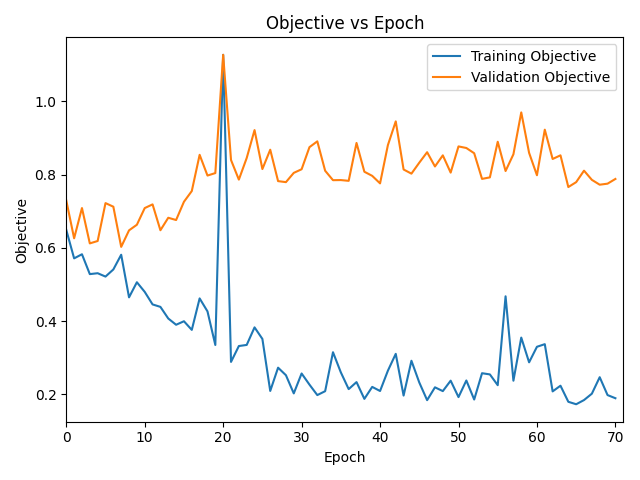
\includegraphics[width=.5\textwidth]{images/exp3/test_model_all_objective.png}}
\caption{Final CrossEntropy Objective vs Epoch for both training and validation datasets}
\label{final_obj}
\end{figure}

\begin{figure}[htbp]
\centerline{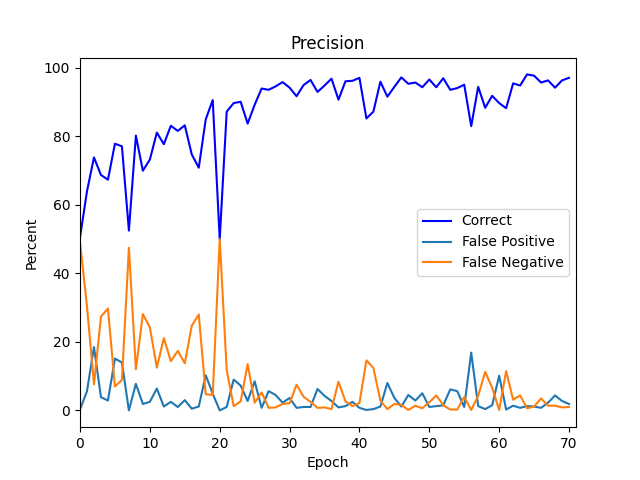
\includegraphics[width=.5\textwidth]{images/exp3/test_model_training.png}}
\caption{Final Accuracy, False Positive, and False Negative vs Epoch for training data}
\label{final_train_acc}
\end{figure}

\begin{figure}[htbp]
\centerline{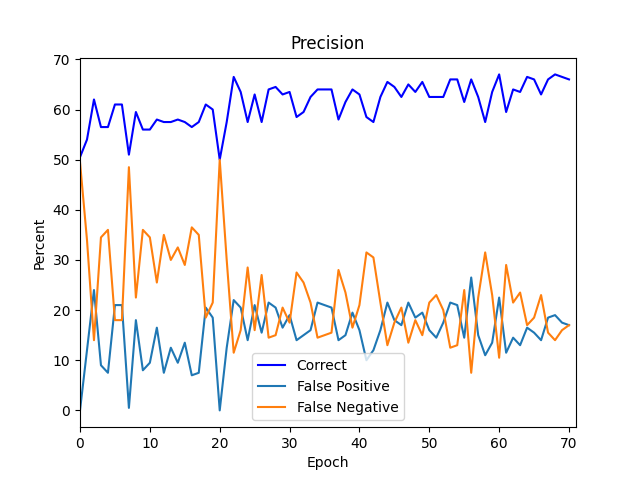
\includegraphics[width=.5\textwidth]{images/exp3/test_model_validation.png}}
\caption{Final Accuracy, False Positive, and False Negative vs Epoch for validation data}
\label{final_valid_acc}
\end{figure}

\begin{table}[htbp]
\caption{Training Statistics for Model in Table~\ref{tab2}}
\begin{center}
\begin{tabular}{|c|c|}
\hline
\textbf{Statistic}&\textbf{Value}\\
\cline{2-2} 
\hline
Final Training J & 0.18967 \\
Final Validatino J & 0.78807 \\
Training Size & (800, 1, 128, 128) \\
Validation Size & (200, 1, 128, 128) \\
Total Epochs & 70 (early termination) \\
Average Batch Time & 4.02 seconds \\
Average Epoch Time & 203.73 seconds \\
Total Training Time & $\sim$4 hours \\
\hline
\end{tabular}
\label{stats1}
\end{center}
\end{table}

\section{Conclusions}

It goes without saying that our team had hoped for a more conclusive and clear result. Among the three of us we tried many different models and variations of each and sharing our results for rapid feedback. In the given time, with the tools we created, we could not forge a model that would exceed 70\% accuracy. On one hand this result is far less than one that could be deemed useful for real-world applications. On the other hand, at 66\% correct, there is promise for refinement to push this process into an applicable place.

\section{Future Work}

The nature of the data had slight pauses in the waveforms, most likely due to short moments between hydraulic pumping and the filtering applied during acquisition. This approach may be successful with data that is more continuous in nature. With a larger set of samples on hand, a larger set of frequencies can be distinguished using an STFFT. Additionally, introducing some concepts from a recurrent neural network (RNN) may give the model a larger view of the data as well.

Furthermore, the data acquisition set up is in the structural testing facility on campus \cite{b10}. Prior work has been conducted to build a live testing set up with edge and cloud computing for real time classification. Therefore, this model could be used for real-time classification of acoustic signals through the edge computing node. Thus, the signals would be classified before propagating to the central cloud. The edge device could be used on board aircraft or affixed on a bridge for live structural monitoring.

Finally, given the image-based approach of the CNN, revisiting this problem with access to properly vectorized and GPU accelerated learning APIs would allow for further experimentation and iteration over the hand-coded tools we had access to for this experiment. 



\begin{thebibliography}{00}
\bibitem{b1} Farhan Tanvir Santo and Tariq Pervez Sattar and Graham Edwards, ``Validation of Acoustic Emission Waveform Entropy as a Damage Identification Feature,'' Applied Sciences, vol. 9, September 2018

\bibitem{b2} Shawn Hershey et. al, ``CNN Architectures for Large-Scale Audio Classification,'' arXiv: 1609.09430 [cs.SD]

\bibitem{b3} Naoya Takahashi and Michael Gygli and Beat Pfister and Luc Van Gool, ``Deep Convolutional Neural Networks and Data Augmentation for Acoustic Event Detection,'' arXiv: 1604.07160v2 [cs.SD]

\bibitem{b4} Sergey Levine and Peter Pastor and Alex Krizhevsky and Deirdre Quillen, ``Learning Hand-Eye Coordination for Robotic Grasping with Deep Learning and Large-Scale Data Collection,'', arXiv:1603.02199v4 [cs.LG]

\bibitem{b5} E1820-20 Standard Test Method for Measurement of Fracture Toughness, ASTM International, West Conshohocken, PA, 2020. 

\bibitem{b6} 647-15e1 Standard Test Method for Measurement of Fatigue Crack Growth Rates, ASTM International, West Conshohocken, PA, 2015. 

\bibitem{b7} C. Cavallo. ``All About 2024 Aluminum (Properties, Strength and Uses)'' Thomasnet. https://www.thomasnet.com/articles/metals-metal-products/2024-aluminum/

\bibitem{b8} E976-15 Standard Guide for Determining the Reproducibility of Acoustic Emission Sensor Response, ASTM International, West Conshohocken, PA, 2015. 

\bibitem{b9} A. A. Pollock, "Acoustic emission inspection," Metals handbook, 1989.

\bibitem{b10} Malik, S., Rouf, R., Mazur, K., \& Kontsos, A. (2020). The Industry Internet of Things (IIoT) as a Methodology for Autonomous Diagnostics in Aerospace Structural Health Monitoring. Aerospace, 7(5), 64.

\end{thebibliography}
\vspace{12pt}



\end{document}
